\documentclass[
  man,
  longtable,
  nolmodern,
  notxfonts,
  notimes,
  colorlinks=true,linkcolor=blue,citecolor=blue,urlcolor=blue]{apa7}

\usepackage{amsmath}
\usepackage{amssymb}




\RequirePackage{longtable}
\RequirePackage{threeparttablex}

\makeatletter
\renewcommand{\paragraph}{\@startsection{paragraph}{4}{\parindent}%
	{0\baselineskip \@plus 0.2ex \@minus 0.2ex}%
	{-.5em}%
	{\normalfont\normalsize\bfseries\typesectitle}}

\renewcommand{\subparagraph}[1]{\@startsection{subparagraph}{5}{0.5em}%
	{0\baselineskip \@plus 0.2ex \@minus 0.2ex}%
	{-\z@\relax}%
	{\normalfont\normalsize\bfseries\itshape\hspace{\parindent}{#1}\textit{\addperi}}{\relax}}
\makeatother




\usepackage{longtable, booktabs, multirow, multicol, colortbl, hhline, caption, array, float, xpatch}
\setcounter{topnumber}{2}
\setcounter{bottomnumber}{2}
\setcounter{totalnumber}{4}
\renewcommand{\topfraction}{0.85}
\renewcommand{\bottomfraction}{0.85}
\renewcommand{\textfraction}{0.15}
\renewcommand{\floatpagefraction}{0.7}

\usepackage{tcolorbox}
\tcbuselibrary{listings,theorems, breakable, skins}
\usepackage{fontawesome5}

\definecolor{quarto-callout-color}{HTML}{909090}
\definecolor{quarto-callout-note-color}{HTML}{0758E5}
\definecolor{quarto-callout-important-color}{HTML}{CC1914}
\definecolor{quarto-callout-warning-color}{HTML}{EB9113}
\definecolor{quarto-callout-tip-color}{HTML}{00A047}
\definecolor{quarto-callout-caution-color}{HTML}{FC5300}
\definecolor{quarto-callout-color-frame}{HTML}{ACACAC}
\definecolor{quarto-callout-note-color-frame}{HTML}{4582EC}
\definecolor{quarto-callout-important-color-frame}{HTML}{D9534F}
\definecolor{quarto-callout-warning-color-frame}{HTML}{F0AD4E}
\definecolor{quarto-callout-tip-color-frame}{HTML}{02B875}
\definecolor{quarto-callout-caution-color-frame}{HTML}{FD7E14}

%\newlength\Oldarrayrulewidth
%\newlength\Oldtabcolsep


\usepackage{hyperref}




\providecommand{\tightlist}{%
  \setlength{\itemsep}{0pt}\setlength{\parskip}{0pt}}
\usepackage{longtable,booktabs,array}
\usepackage{calc} % for calculating minipage widths
% Correct order of tables after \paragraph or \subparagraph
\usepackage{etoolbox}
\makeatletter
\patchcmd\longtable{\par}{\if@noskipsec\mbox{}\fi\par}{}{}
\makeatother
% Allow footnotes in longtable head/foot
\IfFileExists{footnotehyper.sty}{\usepackage{footnotehyper}}{\usepackage{footnote}}
\makesavenoteenv{longtable}

\usepackage{graphicx}
\makeatletter
\newsavebox\pandoc@box
\newcommand*\pandocbounded[1]{% scales image to fit in text height/width
  \sbox\pandoc@box{#1}%
  \Gscale@div\@tempa{\textheight}{\dimexpr\ht\pandoc@box+\dp\pandoc@box\relax}%
  \Gscale@div\@tempb{\linewidth}{\wd\pandoc@box}%
  \ifdim\@tempb\p@<\@tempa\p@\let\@tempa\@tempb\fi% select the smaller of both
  \ifdim\@tempa\p@<\p@\scalebox{\@tempa}{\usebox\pandoc@box}%
  \else\usebox{\pandoc@box}%
  \fi%
}
% Set default figure placement to htbp
\def\fps@figure{htbp}
\makeatother


% definitions for citeproc citations
\NewDocumentCommand\citeproctext{}{}
\NewDocumentCommand\citeproc{mm}{%
  \begingroup\def\citeproctext{#2}\cite{#1}\endgroup}
\makeatletter
 % allow citations to break across lines
 \let\@cite@ofmt\@firstofone
 % avoid brackets around text for \cite:
 \def\@biblabel#1{}
 \def\@cite#1#2{{#1\if@tempswa , #2\fi}}
\makeatother
\newlength{\cslhangindent}
\setlength{\cslhangindent}{1.5em}
\newlength{\csllabelwidth}
\setlength{\csllabelwidth}{3em}
\newenvironment{CSLReferences}[2] % #1 hanging-indent, #2 entry-spacing
 {\begin{list}{}{%
  \setlength{\itemindent}{0pt}
  \setlength{\leftmargin}{0pt}
  \setlength{\parsep}{0pt}
  % turn on hanging indent if param 1 is 1
  \ifodd #1
   \setlength{\leftmargin}{\cslhangindent}
   \setlength{\itemindent}{-1\cslhangindent}
  \fi
  % set entry spacing
  \setlength{\itemsep}{#2\baselineskip}}}
 {\end{list}}
\usepackage{calc}
\newcommand{\CSLBlock}[1]{\hfill\break\parbox[t]{\linewidth}{\strut\ignorespaces#1\strut}}
\newcommand{\CSLLeftMargin}[1]{\parbox[t]{\csllabelwidth}{\strut#1\strut}}
\newcommand{\CSLRightInline}[1]{\parbox[t]{\linewidth - \csllabelwidth}{\strut#1\strut}}
\newcommand{\CSLIndent}[1]{\hspace{\cslhangindent}#1}





\usepackage{newtx}

\defaultfontfeatures{Scale=MatchLowercase}
\defaultfontfeatures[\rmfamily]{Ligatures=TeX,Scale=1}





\title{The Cuteness Fallacy: How Visual Representations Influence
Knowledge Acquisition About Ecological Threats of Domestic Cats}


\shorttitle{The Cuteness Fallacy}


\usepackage{etoolbox}






\author{Arash Sal Moslehian}



\affiliation{
{Neuro-X, EPFL}}




\leftheader{Moslehian}



\abstract{Despite being beloved pets, cats pose significant threats to
wildlife through predation and competition. Existing legislations
struggle to mitigate these impacts, highlighting the need for effective
communication strategies. This study surveyed 150 university students to
investigate how different visual representations of domestic
cats---categorized as cute, scary, dirty, or neutral---affect recall of
positive, negative, or neutral information about cats. We hypothesized
that negative and dirty representations would enhance recall of negative
information, while cute representations would enhance positive recall.
Contrary to expectations, no significant effect of visual
representations on information recall was found. Results suggest strong
emotional bonds with cats may buffer negative imagery. Exploratory
analyses indicated that individual factors, like having a cat allergy,
reduced recall of positive information. These findings show the
complexity of altering public perception about positively perceived
animals like cats.}

\keywords{biodiversity, cats, memory, emotions, representation}

\authornote{ 

\par{     The author would like to thank Oliver Smedt, Andrey Shusharin
and Valentine Rehn for their help with survey and data annotation. I
further thank Maël Theubet for their guidance throughout the study.  }
\par{Correspondence concerning this article should be addressed to Arash
Sal Moslehian, Email: arash.salmoslehian@epfl.ch}
}

\makeatletter
\let\endoldlt\endlongtable
\def\endlongtable{
\hline
\endoldlt
}
\makeatother
\RequirePackage{longtable}
\DeclareDelayedFloatFlavor{longtable}{table}

\urlstyle{same}



\usepackage{booktabs}
\usepackage{longtable}
\usepackage{array}
\usepackage{multirow}
\usepackage{wrapfig}
\usepackage{float}
\usepackage{colortbl}
\usepackage{pdflscape}
\usepackage{tabu}
\usepackage{threeparttable}
\usepackage{threeparttablex}
\usepackage[normalem]{ulem}
\usepackage{makecell}
\usepackage{xcolor}
\makeatletter
\@ifpackageloaded{caption}{}{\usepackage{caption}}
\AtBeginDocument{%
\ifdefined\contentsname
  \renewcommand*\contentsname{Table of contents}
\else
  \newcommand\contentsname{Table of contents}
\fi
\ifdefined\listfigurename
  \renewcommand*\listfigurename{List of Figures}
\else
  \newcommand\listfigurename{List of Figures}
\fi
\ifdefined\listtablename
  \renewcommand*\listtablename{List of Tables}
\else
  \newcommand\listtablename{List of Tables}
\fi
\ifdefined\figurename
  \renewcommand*\figurename{Figure}
\else
  \newcommand\figurename{Figure}
\fi
\ifdefined\tablename
  \renewcommand*\tablename{Table}
\else
  \newcommand\tablename{Table}
\fi
}
\@ifpackageloaded{float}{}{\usepackage{float}}
\floatstyle{ruled}
\@ifundefined{c@chapter}{\newfloat{codelisting}{h}{lop}}{\newfloat{codelisting}{h}{lop}[chapter]}
\floatname{codelisting}{Listing}
\newcommand*\listoflistings{\listof{codelisting}{List of Listings}}
\makeatother
\makeatletter
\makeatother
\makeatletter
\@ifpackageloaded{caption}{}{\usepackage{caption}}
\@ifpackageloaded{subcaption}{}{\usepackage{subcaption}}
\makeatother

% From https://tex.stackexchange.com/a/645996/211326
%%% apa7 doesn't want to add appendix section titles in the toc
%%% let's make it do it
\makeatletter
\xpatchcmd{\appendix}
  {\par}
  {\addcontentsline{toc}{section}{\@currentlabelname}\par}
  {}{}
\makeatother

%% Disable longtable counter
%% https://tex.stackexchange.com/a/248395/211326

\usepackage{etoolbox}

\makeatletter
\patchcmd{\LT@caption}
  {\bgroup}
  {\bgroup\global\LTpatch@captiontrue}
  {}{}
\patchcmd{\longtable}
  {\par}
  {\par\global\LTpatch@captionfalse}
  {}{}
\apptocmd{\endlongtable}
  {\ifLTpatch@caption\else\addtocounter{table}{-1}\fi}
  {}{}
\newif\ifLTpatch@caption
\makeatother

\begin{document}

\maketitle


\setcounter{secnumdepth}{-\maxdimen} % remove section numbering

\setlength\LTleft{0pt}


\section{Introduction}\label{introduction}

The comforting purr of our beloved cats is masking a silent threat to
biodiversity, one of the most urgent worldwide challenges today
(\citeproc{ref-watson2019summary}{Watson et al., 2019}). Although
domestic cats are the most popular pets in Europe
(\citeproc{ref-statista2022eu}{Statista, 2023}), their impact on
wildlife, particularly on birds, is a cause for great concern. They are
responsible for the annual death of 30 million birds in Switzerland
(\citeproc{ref-question2021}{National~Council~of~Switzerland, 2021}) and
are the leading cause of death, comparable to window collisions, in
Belgium and France (\citeproc{ref-pavisse2019domestic}{Pavisse et al.,
2019}). These impacts also extend beyond predation and include
competition (\citeproc{ref-george1974domestic}{George, 1974}), fear
effect, disease transmission (\citeproc{ref-loss2017population}{Loss \&
Marra, 2017}), and hybridization
(\citeproc{ref-macdonald2010biology}{Macdonald \& Loveridge, 2010}).
Many legislations at the national and international levels exist to
address biodiversity concerns, such as not allowing owned cats to go
outdoors or manually removing unowned and stray cats from the landscape.
The implementation of these laws, however, proves to be challenging
(\citeproc{ref-trouwborst2020domestic}{Trouwborst et al., 2020}),
implying that addressing this issue requires not only legal enforcement
but also a collective effort from pet owners and the public. In this
study, we would like to see if it is possible to affect people's
knowledge acquisition of information about cats using different
representations of cats that may trigger their internal bias. For
example, when humans encounter a potentially threatening animal, there
is an evolutionary advantage in processing negative information about
the creature more attentively, a phenomenon which is a form of
negativity bias (\citeproc{ref-rozin2001negativity}{Rozin \& Royzman,
2001}). If this is the case, we would then be able to better inform the
public about the detrimental impacts of domestic cats on biodiversity
and increase awareness in the hopes that it will encourage individuals
to take action, rather than solely relying on governmental regulations.

A prior study has demonstrated that participants exposed to images of
bats portrayed as threatening creatures tended to recall more negative
information about bats compared to alternative representations
(\citeproc{ref-greving2020better}{Greving \& Kimmerle, 2020a}). Another
study has shown that representing animals as distressed could serve as a
way to evoke different emotions and attitudes towards wildlife
conservation (\citeproc{ref-greving2021you}{Greving \& Kimmerle, 2021}).
There, however, exists a distinct lack of research regarding the
application of the negativity bias to domestic cats and their influence
on biodiversity. Unlike bats, domestic cats are considered pets and have
an overwhelmingly cute perception among people. Cats are also a common
presence in households in Europe, making their impact on wildlife
pervasive and immediate.

The present study seeked to address this gap by exploring how different
visual representations of cats can influence participants' recall of
information about cats. Participants were tasked with reading a text
about cats while being presented with images of cats, each falling into
categories of scary, dirty, cute, or neutral (in which they are shown no
image). Unlike the previous study that utilized imperiled as a category,
we opted to add dirty instead since cats already provoke feelings of
compassion in people and our hypothesis focuses more on negative
representations. The dirty representation also allows us to explore the
influence of disgust which is a powerful emotion that not only triggers
a strong immediate response but also has a lasting impact on our
cognitive processes. The importance of disgust lies in its evolutionary
role in protecting us from harmful substances and pathogens, which is
why it is closely linked to memory recall
(\citeproc{ref-schienle2021disgust}{Schienle et al., 2021}). Disgust has
also been shown to cause increased memory recall compared to equally
unpleasant frightening images
(\citeproc{ref-croucher2011disgust}{Croucher et al., 2011}). As
suggested by the authors of the prevous study
(\citeproc{ref-greving2020better}{Greving \& Kimmerle, 2020a}), we
included both free recall and recognition tasks as different measures to
assess knowledge acquisition. Given that cats are more familiar as pets,
we anticipated a more positive information recall with cute
representations, despite the minimal impact of cute representation in
the previous study (\citeproc{ref-greving2020better}{Greving \&
Kimmerle, 2020a}). We also hypothesized that scary or dirty cat pictures
increase the recall of negative information compared to other
representations. These finding may be crucial for changing attitudes
toward cats by effectively informing and influencing public perception
and behavior through targeted, impactful communication strategies.

\section{Methods and Material}\label{methods-and-material}

\subsection{Participants}\label{participants}

The participants for the study were recruited both through personal
contacts and through the University of Lausanne (UNIL). Those recruited
through personal contacts participated without compensation, while those
recruited through the UNIL were compensated with university credits. In
total, there were 150 participants. They were mostly Swiss (66.33\%) and
primarily young female students (78.72\%). The primary fields of study
of the participants were Psychology (84\%) and Physics (8\%). Out of the
participants, (47\%) reported their level of English as B2 or above. The
mean age was 21.3 years (\(SD = 3.02\), range \(18-47\)). The
participants were informed about the usage of their anonymized data.

\subsection{Survey Procedure}\label{survey-procedure}

The aim of the survey was to record participants' recollection of cat
information after having looked at a variety of pictures of cats. The
study was conducted anonymously online using the survey tool Qualtrics.
After consenting to the terms of the survey the participant was
instructed to provide their age, sex, field of study/occupation, if they
have a cat allergy, if they have owned a cat, how much they considered
themselves a city person (cityness), their nationality, and their level
of English. The participants were then shown a picture of a cat from one
of four categories cute, scary, dirty and neutral (neutral meant no
picture was shown) Figure~\ref{fig-cats}. If a picture was shown, they
were asked to answer two question regarding the picture to assess their
attention. Participants that failed the attention check were removed
from the study entirely.

They were then prompted to read a text with information (positive,
negative, neutral), accompanied by the same picture. Upon finishing the
text they were prompted to complete two memory tests. The first was a
free recall test, in which they were asked to provide three pieces of
information that they remember from the text. In the second recall test,
they were prompted to answer yes and no to whether certain words had
appeared in the text
(\citeproc{ref-nickreidTrueFalseRecognition2023}{Nick Reid \& Jamieson,
2023}). Of these words 12 were positive, 12 were negative, 6 were
neutral and 15 were not in the text (unrelated). After completing this
recall test, the participant was prompted to redo the survey with a new
text and a different condition. After the second trial, the participant
was thanked, and debriefed on the purpose of the study. An overview of
the survey flow can be seen on Figure~\ref{fig-flow}.

\begin{figure}[H]

\caption{\label{fig-cats}Different conditions of the study.}

\begin{minipage}{0.50\linewidth}

\subcaption{\label{fig-cats-scary}Scary}

\centering{

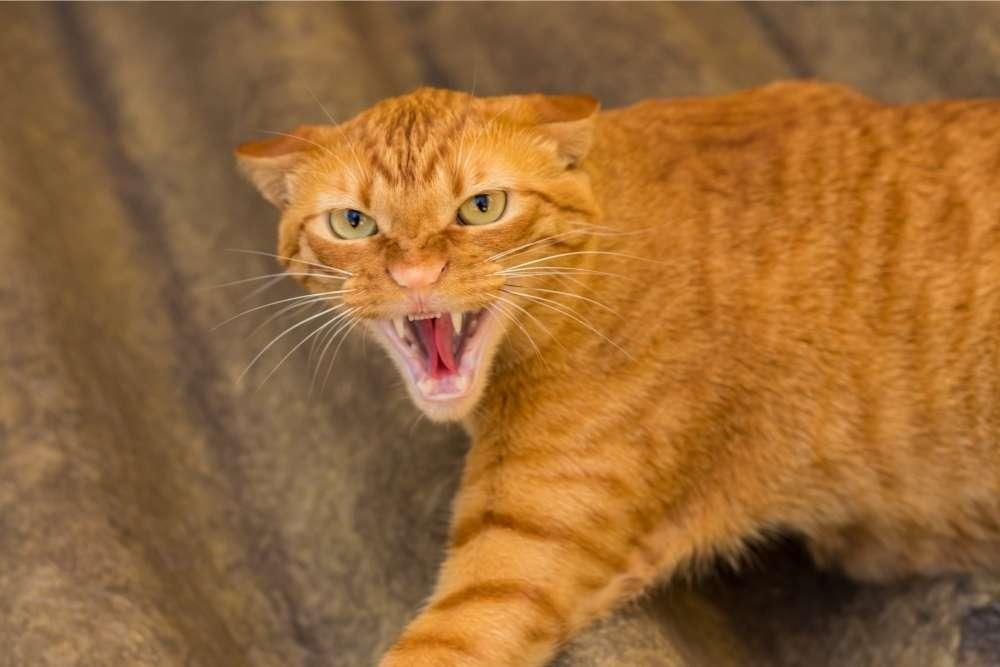
\includegraphics[width=2.08333in,height=\textheight,keepaspectratio]{assets/scary.jpg}

}

\end{minipage}%
%
\begin{minipage}{0.50\linewidth}

\subcaption{\label{fig-cats-dirty}Dirty}

\centering{

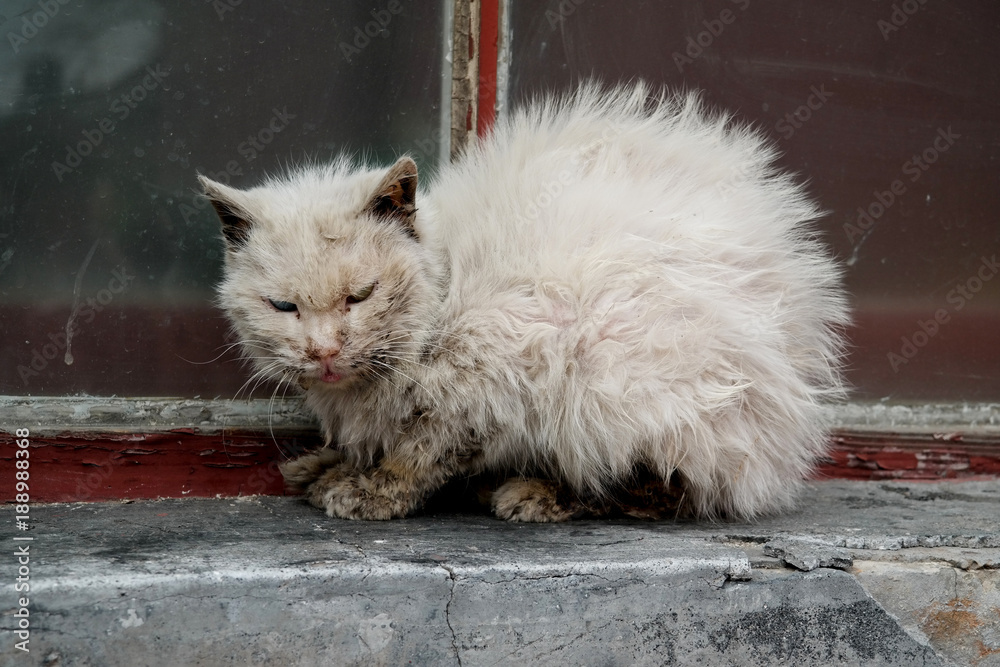
\includegraphics[width=2.08333in,height=\textheight,keepaspectratio]{assets/dirty.jpg}

}

\end{minipage}%
\newline
\begin{minipage}{\linewidth}

\subcaption{\label{fig-cats-cute}Cute}

\centering{

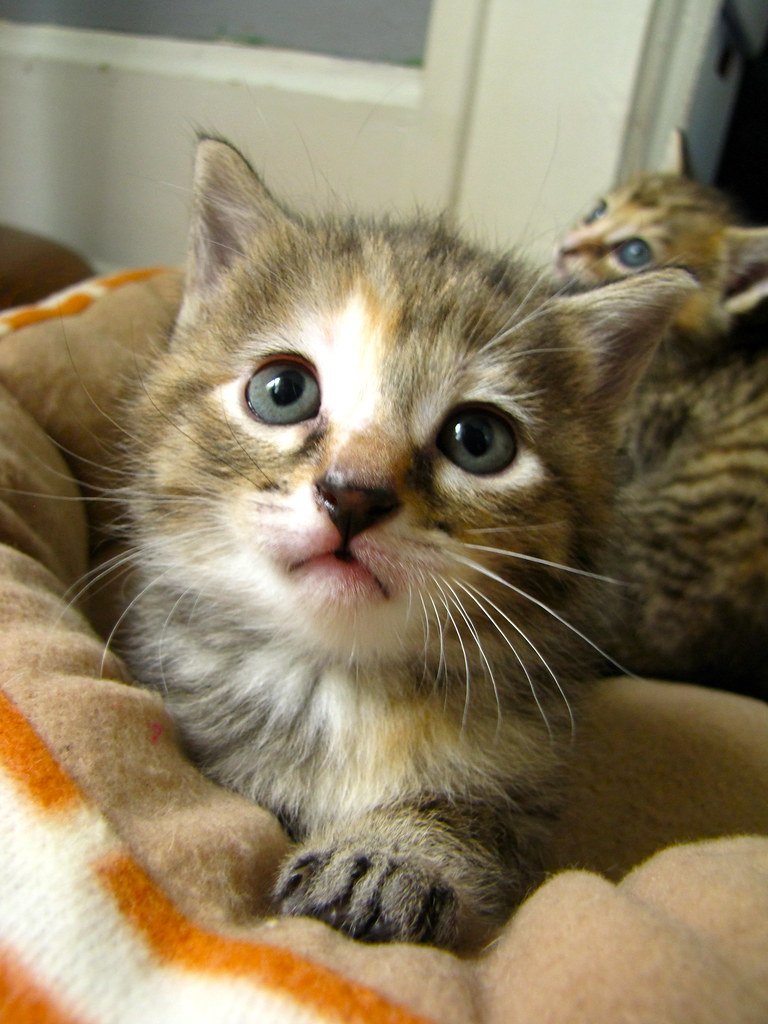
\includegraphics[width=\linewidth,height=2.08333in,keepaspectratio]{assets/cute.jpg}

}

\end{minipage}%

\end{figure}%

\begin{figure}[H]

\caption{\label{fig-flow}Procedure of study.}

\centering{

\pandocbounded{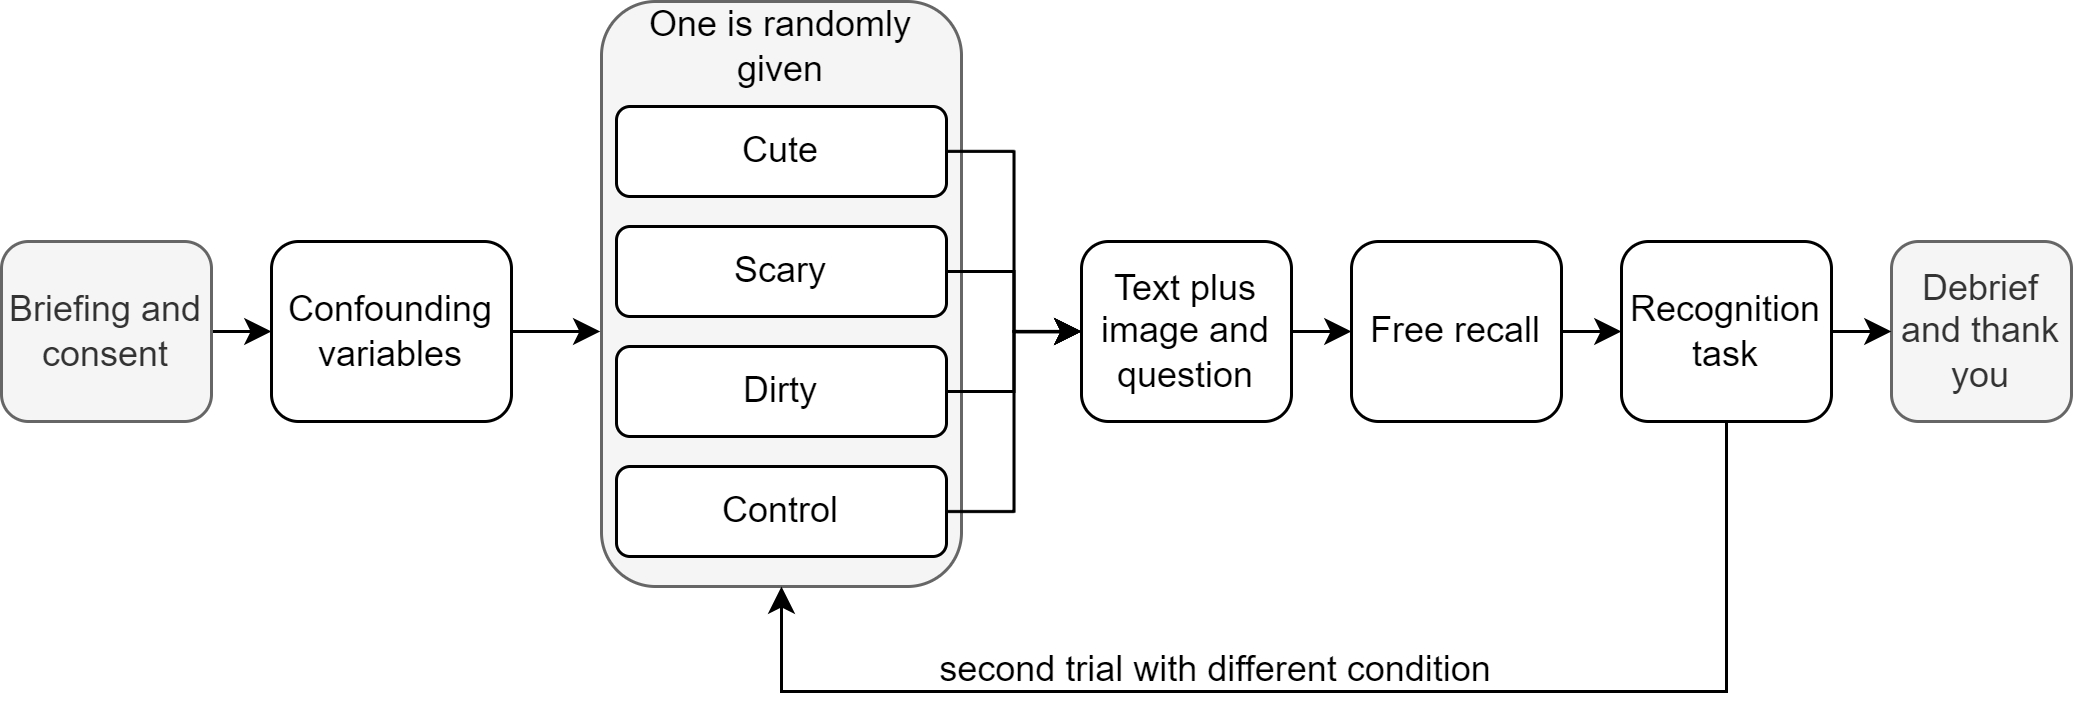
\includegraphics[keepaspectratio]{assets/flowchart.jpg}}

}

\end{figure}%

\subsection{Data Prepration and
Analysis}\label{data-prepration-and-analysis}

The amount of positive, negative, neutral, and unrelated information for
the free recall task was manually annotated by systematically comparing
what was recalled by the participant with a schema of all the
information contained in the text listed as positive, neutral and
negative. Each text response by the participant was reviewed twice, by
two different reviewers, the results of which were then averaged. From
the recognition task, the fraction of positive, negative, neutral and
unrelated recalled keywords were calculated.

The study was conducted twice by each participant, with two different
conditions. To later check for possible dependency between the two
trials, a categorical variable was added to the dataset specifying which
condition the participant was put through, before the current condition.
For the entries corresponding to the first trial this variable had the
value none, and for entries corresponding to the second trial, this
variable was assigned the condition on the first trial (either cute,
dirty, scary, neutral).

The data were cleaned using Python (\citeproc{ref-van2007python}{Van
Rossum et al., 2007}) and analyzed using R (\citeproc{ref-r2013r}{R Core
Team et al., 2013}). For the main analysis since we had clear
well-defined hypothesis, we used orthogonal contrast analyses, which
test a priori hypotheses, simplify result interpretation, reduce type I
error, and increase statistical power. For k levels of a categorical
variable (in our case, four), we needed k -- 1 contrasts. Each contrast
must have coefficients summing to zero, and the sum of the products of
coefficients across contrasts must also be zero
(\citeproc{ref-nogueiraOrthogonalContrastsDefinitions2004}{Nogueira,
2004}). As exploratory measures, we next performed ANOVA to test for any
difference in recalled information in between the different conditions.
Afterward, to evaluate the impact of covariates, we utilized the
stepwise selection method provided by the MASS package
(\citeproc{ref-venablesModernAppliedStatistics2002}{Venables \& Ripley,
2002}) in R, focusing on minimizing the Akaike Information Criterion
(AIC). The AIC is a well-established metric used to assess the relative
quality of statistical models for a given dataset, balancing model fit
and complexity. By employing this method in a bidirectional manner, we
aimed to identify the optimal set of variables that yield the best
predictive model while maintaining parsimony. For each memory
recognition measure, we found variables that significantly contributed
to the model's explanatory power. The initial model for the stepwise
process contained variables condition, previous condition (this is only
valid for the second round), age, study level, field of study, having a
cat allergy, having previously had a cat, how much the participant feels
they are a city person, nationality, and level of English language.

\section{Results}\label{results}

The planned contrasts for each hypothesis are shown in
Table~\ref{tbl-contrasts}. Orthogonal contrasts analysis revealed no
significant effect for any of the contrasts in any of the neutral,
positive, negative, and unrelated information retrieval for both free
recall Table~\ref{tbl-contrasts-freerecall} and recognition memory tests
Table~\ref{tbl-contrasts-recog}. The first contrast, related to the
hypothesis that cute representation elicits more positive information
retrieval, was not supported by the data. Similarly, the second
contrast, which hypothesized that scary representation elicits more
negative information retrieval, showed no significant effects.
Additionally, the third contrast, which hypothesized that dirty
representation elicits more negative information retrieval compared to
cute and neutral, also did not yield significant results. Thus, these
findings overall do not support any of our three hypotheses. To see if
there are any differences in between the means of our conditions, we
next performed ANOVA on each memory tasks. There were no significant
difference in between the means within free recall task
Table~\ref{tbl-anova-freerecall} and recognition memory task
Table~\ref{tbl-anova-recog}. Therefore, we did not perform any further
post-hoc analysis. Finally, to explore the effect of covariates on the
prediction, we tried to find the best predicting model for free recall
Table~\ref{tbl-aic-freerecall} and recognition memory
Table~\ref{tbl-aic-recog} task based on all the covariates.
Interestingly, the condition variable was removed by the stepwise
process from all the models and manually including it made the
performance of the model worse. These results also indicate that putting
the participants through the trial two times, which is reflected in the
``Previous.condition'' variable has no effect on the prediction of
recognition memory task. Moreover, we found that having an allergy
significantly improved the model for predicting the amount of positive
information in recognition task with a negative coefficient
Table~\ref{tbl-sig-covar} meaning, having an allergy with cat makes you
recall less positive information.

\section{Discussion}\label{discussion}

This study explored how different visual representations of cats
influence participants' recall of information about cats. The findings
of our study provide valuable insights into the complexity of
influencing public perception and knowledge acquisition. We had hoped on
the potential of triggering internal biases in participants through
images categorized as cute, scary, dirty, or neutral. However, contrary
to our hypotheses, the different visual representations of cats did not
significantly affect the recall of positive, negative, or neutral
information about cats.

These findings are not in line with previous research that demonstrated
the influence of visual representations on knowledge acquisition about
bats (\citeproc{ref-bats}{Greving \& Kimmerle, 2020b}). They found that
portraying bats as threatening increased the recall of negative
information, aligning with an evolutionary advantage in processing
negative information about potentially dangerous animals. However, this
study's results suggest that this phenomenon may not extend to domestic
cats. This discrepancy can be attributed to the unique social and
emotional bonds humans share with domestic cats, which likely buffer
against the effects of negative representations. Additionally, the
familiarity and frequent positive interactions with cats may overshadow
attempts to show their ecological impact through negative imagery.

The overwhelming prevalence of cute representations of cats in popular
culture (\citeproc{ref-thibault2018run}{Thibault \& Marino, 2018}) may
have attenuated the influence of other representations on participants'
information recall. Additionally, the emotional valence associated with
each representation may not have been strong or distinct enough to
elicit differential recall of information. While previous studies have
shown the influence of emotions like fear and disgust on memory recall
(\citeproc{ref-croucher2011disgust}{Croucher et al., 2011}), these
effects may vary depending on individual differences and contextual
factors. Another study that tried to influence knowledge acquisition of
participants using the image of a cute fox, also did not find an overall
effect of visual emotionalization on knowledge gain which they found
surprising (\citeproc{ref-flemming2018emotionalization}{Flemming et al.,
2018}).

Our exploratory analyses revealed that demographic factors such as
having a cat allergy influenced the recall of information, specifically
reducing the recall of positive information. Participants with cat
allergies recalled less positive information in the recognition task.
This suggests that personal experiences with cats may influence
information recall independently of the visual representations. This
shows that targeted communication strategies might need to consider
individual differences more closely.

Our study contributes to the growing body of literature on human-animal
interactions and the role of visual representations in shaping knowledge
and attitudes (\citeproc{ref-altmeyer2020use}{Altmeyer et al., 2020}).
While previous research has demonstrated the effectiveness of negative
representations in increasing knowledge recall about less familiar and
more negatively perceived animals, our study shows the limitations of
applying similar strategies to more positively perceived animals, like
cats. Moving forward, researchers may explore alternative strategies for
enhancing public awareness of biodiversity threats posed by domestic
cats, considering factors such as individual differences, cultural
influences, and message framing.

\subsection{Limitations}\label{limitations}

Several limitations in our study warrant consideration. First, the
sample size was relatively small and predominantly composed of young,
Swiss female psychology students, which may limit the generalizability
of our findings to broader populations. Second, the study's reliance on
self-reported data and online survey methods introduces potential
biases, such as social desirability and varying levels of participant
engagement (\citeproc{ref-caputo2017social}{Caputo, 2017}). Although
attention checks were implemented, they may not entirely mitigate these
biases (\citeproc{ref-kung2018attention}{Kung et al., 2018}). Third, the
study design involved short-term exposure to visual stimuli and only
considered immediate recall after exposure, which may not be sufficient
to produce lasting changes in perception or knowledge
(\citeproc{ref-postle2015cognitive}{Postle, 2015}). Additionally, our
study did not account for the potential influence of pre-existing
attitudes towards cats and wildlife conservation. Participants with
strong pre-existing beliefs may be less susceptible to change through
visual manipulation alone. Finally, while the study aimed to explore the
negativity bias by using dirty and scary representations, the selected
images may not have been sufficiently impactful to elicit strong
negative responses.

\subsection{Future Directions}\label{future-directions}

In future studies, enhancing the generalizability of findings should be
a priority by incorporating a more diverse and larger sample.
Furthermore, investigations beyond visual representations and towards
other sensory modalities or combinations of representations could
provide valuable insights into information recall. Additionally,
considering and controlling for baseline attitudes towards cats, would
improve the understanding of the observed effects. Moreover, rigorous
pre-testing and selection of images are essential to ensure they
reliably evoke intended emotional responses. Lastly, investigating
long-term recall is crucial to make see the impact of visual
representations over time.

\section{Conclusion}\label{conclusion}

This study explored how different visual representations of cats (cute,
scary, dirty, or neutral) affect positive, negative, and neutral
information recall about cats. Contrary to our hypotheses, these
representations did not significantly influence recall. This suggests
that strong emotional bonds with domestic cats may mitigate the effects
of negative imagery. Individual factors, such as cat allergies,
influenced recall, reducing positive information recall. This shows the
need to consider personal differences in awareness campaigns about the
ecological impact of cats. Our findings suggest that while visual
representations work for less familiar animals like bats, they are less
effective for familiar, positively perceived animals like cats. Future
research should explore alternative methods and individual differences
to improve public awareness efforts.

\begin{table}

{\caption{{Planned contrasts.}{\label{tbl-contrasts}}}
\vspace{-20pt}}

\begin{longtable}[]{@{}lrrrr@{}}
\toprule\noalign{}
Hypothesis & Cute & Neutral & Dirty & Scary \\
\midrule\noalign{}
\endhead
\bottomrule\noalign{}
\endlastfoot
Cute vs Rest & 3 & -1 & -1 & -1 \\
Scary vs Rest & -1 & -1 & -1 & 3 \\
Dirty vs (Cute and Neut) & -1 & -1 & 2 & 0 \\
\end{longtable}

\end{table}

\begin{table}

{\caption{{Orthogonal contrasts regression analysis for recognition
memory tasks.}{\label{tbl-contrasts-recog}}}
\vspace{-20pt}}

\begin{longtable*}[t]{lllll}
\toprule
Term & Estimate & SE & 95 \% CI & p\\
\midrule
\addlinespace[0.3em]
\multicolumn{5}{l}{\textbf{Positive information recall}}\\
\hspace{1em}Cute vs Rest & -0.012 & 0.009 & -0.03, 0.006 & .189\\
\hspace{1em}Scary vs Rest & -0.004 & 0.008 & -0.019, 0.011 & .582\\
\hspace{1em}Dirty vs (Cute and Neut) & -0.015 & 0.012 & -0.038, 0.008 & .206\\
\addlinespace[0.3em]
\multicolumn{5}{l}{\textbf{Negative information recall}}\\
\hspace{1em}Cute vs Rest & -0.009 & 0.009 & -0.026, 0.009 & .323\\
\hspace{1em}Scary vs Rest & -0.004 & 0.007 & -0.019, 0.01 & .557\\
\hspace{1em}Dirty vs (Cute and Neut) & -0.009 & 0.011 & -0.032, 0.013 & .423\\
\addlinespace[0.3em]
\multicolumn{5}{l}{\textbf{Neutral information recall}}\\
\hspace{1em}Cute vs Rest & -0.011 & 0.011 & -0.032, 0.01 & .313\\
\hspace{1em}Scary vs Rest & 0.009 & 0.009 & -0.009, 0.027 & .331\\
\hspace{1em}Dirty vs (Cute and Neut) & -0.012 & 0.014 & -0.04, 0.015 & .375\\
\addlinespace[0.3em]
\multicolumn{5}{l}{\textbf{Unrelated information recall}}\\
\hspace{1em}Cute vs Rest & 0.001 & 0.008 & -0.014, 0.016 & .861\\
\hspace{1em}Scary vs Rest & 0.006 & 0.006 & -0.006, 0.019 & .319\\
\hspace{1em}Dirty vs (Cute and Neut) & 0.002 & 0.01 & -0.018, 0.021 & .86\\
\bottomrule
\end{longtable*}

\end{table}

\begin{table}

{\caption{{Orthogonal contrasts regression analysis for free recall
memory tasks.}{\label{tbl-contrasts-freerecall}}}
\vspace{-20pt}}

\begin{longtable*}[t]{lllll}
\toprule
Term & Estimate & SE & 95 \% CI & p\\
\midrule
\addlinespace[0.3em]
\multicolumn{5}{l}{\textbf{Positive information recall}}\\
\hspace{1em}Cute vs Rest & -0.056 & 0.033 & -0.122, 0.01 & .096\\
\hspace{1em}Scary vs Rest & 0.005 & 0.028 & -0.051, 0.061 & .851\\
\hspace{1em}Dirty vs (Cute and Neut) & -0.022 & 0.044 & -0.108, 0.064 & .615\\
\addlinespace[0.3em]
\multicolumn{5}{l}{\textbf{Negative information recall}}\\
\hspace{1em}Cute vs Rest & -0.027 & 0.028 & -0.081, 0.027 & .323\\
\hspace{1em}Scary vs Rest & -0.023 & 0.023 & -0.069, 0.023 & .322\\
\hspace{1em}Dirty vs (Cute and Neut) & -0.064 & 0.036 & -0.134, 0.007 & .077\\
\addlinespace[0.3em]
\multicolumn{5}{l}{\textbf{Neutral information recall}}\\
\hspace{1em}Cute vs Rest & 0.001 & 0.02 & -0.038, 0.04 & .969\\
\hspace{1em}Scary vs Rest & -0.01 & 0.017 & -0.043, 0.024 & .566\\
\hspace{1em}Dirty vs (Cute and Neut) & 0.039 & 0.026 & -0.011, 0.09 & .128\\
\addlinespace[0.3em]
\multicolumn{5}{l}{\textbf{Unrelated information recall}}\\
\hspace{1em}Cute vs Rest & 0.005 & 0.009 & -0.012, 0.021 & .587\\
\hspace{1em}Scary vs Rest & 0.01 & 0.007 & -0.005, 0.024 & .188\\
\hspace{1em}Dirty vs (Cute and Neut) & 0.011 & 0.011 & -0.011, 0.033 & .322\\
\bottomrule
\end{longtable*}

\end{table}

\begin{table}

{\caption{{ANOVA analysis for recognition memory
tasks.}{\label{tbl-anova-recog}}}
\vspace{-20pt}}

\begin{longtable}[]{@{}llll@{}}
\toprule\noalign{}
Information & DF & F & p \\
\midrule\noalign{}
\endhead
\bottomrule\noalign{}
\endlastfoot
Positive information recall & 3, 296 & 0.749 & .523 \\
Negative information recall & 3, 296 & 0.389 & .761 \\
Neutral information recall & 3, 296 & 1.121 & .341 \\
Unrelated information recall & 3, 296 & 0.349 & .79 \\
\end{longtable}

\end{table}

\begin{table}

{\caption{{ANOVA analysis for free recall memory
tasks.}{\label{tbl-anova-freerecall}}}
\vspace{-20pt}}

\begin{longtable}[]{@{}llll@{}}
\toprule\noalign{}
Information & DF & F & p \\
\midrule\noalign{}
\endhead
\bottomrule\noalign{}
\endlastfoot
Positive information recall & 3, 296 & 1.221 & .302 \\
Negative information recall & 3, 296 & 1.201 & .309 \\
Neutral information recall & 3, 296 & 1.138 & .334 \\
Unrelated information recall & 3, 296 & 0.806 & .492 \\
\end{longtable}

\end{table}

\begin{table}

{\caption{{Model selection based on AIC for recognition memory tasks.
\newline{}}{\label{tbl-aic-recog}}}
\vspace{-20pt}}

\begin{threeparttable}
\begin{tabular}[t]{lrrlrr}
\toprule
Model & Df & LR & p & AIC & $R^2$\\
\midrule
\addlinespace[0.3em]
\multicolumn{6}{l}{\textbf{Positive information recall}}\\
\hspace{1em}Full$^1$ & 45 & 47.289 & .497 & -18.269 & 0.146\\
\hspace{1em}AIC Selected$^2$ & 4 & 6.214 & .105 & -59.194 & 0.020\\
\addlinespace[0.3em]
\multicolumn{6}{l}{\textbf{Negative information recall}}\\
\hspace{1em}Full$^1$ & 45 & 44.903 & .591 & -38.586 & 0.139\\
\hspace{1em}AIC Selected$^3$ & 2 & 2.027 & .156 & -81.711 & 0.007\\
\addlinespace[0.3em]
\multicolumn{6}{l}{\textbf{Neutral information recall}}\\
\hspace{1em}Full$^1$ & 45 & 52.788 & .298 & 79.025 & 0.161\\
\hspace{1em}AIC Selected$^4$ & 1 & 0.000 & - & 43.813 & 0.000\\
\addlinespace[0.3em]
\multicolumn{6}{l}{\textbf{Unrelated information recall}}\\
\hspace{1em}Full$^1$ & 45 & 58.238 & .155 & -134.357 & 0.176\\
\hspace{1em}AIC Selected$^5$ & 10 & 24.144 & .005 & -170.263 & 0.077\\
\bottomrule
\end{tabular}
\begin{tablenotes}
\item[1] Condition, Previous.condition, Age , Study.level, Field.of.study, Allergy, Had.cats.previously, Cityness, Nationality, English.level
\item[2] Allergy, Had.cats.previously
\item[3] Cityness
\item[4] Intercept
\item[5] Age, Field.of.study, Allergy, Had.cats.previously, Cityness
\end{tablenotes}
\end{threeparttable}

\end{table}

\begin{table}

{\caption{{Model selection based on AIC for free recall memory tasks.
\newline{}}{\label{tbl-aic-freerecall}}}
\vspace{-20pt}}

\begin{threeparttable}
\begin{tabular}[t]{lrrlrr}
\toprule
Model & Df & LR & p & AIC & $R^2$\\
\midrule
\addlinespace[0.3em]
\multicolumn{6}{l}{\textbf{Positive information recall}}\\
\hspace{1em}Full$^1$ & 45 & 30.012 & .975 & 783.103 & 0.095\\
\hspace{1em}AIC Selected$^2$ & 1 & 0.000 & - & 725.115 & 0.000\\
\addlinespace[0.3em]
\multicolumn{6}{l}{\textbf{Negative information recall}}\\
\hspace{1em}Full$^1$ & 45 & 37.048 & .861 & 658.310 & 0.116\\
\hspace{1em}AIC Selected$^3$ & 7 & 15.008 & .022 & 604.349 & 0.049\\
\addlinespace[0.3em]
\multicolumn{6}{l}{\textbf{Neutral information recall}}\\
\hspace{1em}Full$^1$ & 45 & 98.536 & <.001 & 401.509 & 0.280\\
\hspace{1em}AIC Selected$^4$ & 27 & 84.677 & <.001 & 379.368 & 0.246\\
\addlinespace[0.3em]
\multicolumn{6}{l}{\textbf{Unrelated information recall}}\\
\hspace{1em}Full$^1$ & 45 & 44.421 & .61 & -54.895 & 0.138\\
\hspace{1em}AIC Selected$^5$ & 3 & 8.534 & .015 & -103.007 & 0.028\\
\bottomrule
\end{tabular}
\begin{tablenotes}
\item[1] Condition, Previous.condition, Age , Study.level, Field.of.study, Allergy, Had.cats.previously, Cityness, Nationality, English.level
\item[2] Intercept
\item[3] Previous.condition, Study.level
\item[4] Previous.condition, Study.level, Nationality
\item[5] Allergy
\end{tablenotes}
\end{threeparttable}

\end{table}

\begin{table}

{\caption{{Effect of having an allergy on positive information recall in
recognition task.}{\label{tbl-sig-covar}}}
\vspace{-20pt}}

\begin{longtable}[]{@{}lllll@{}}
\toprule\noalign{}
Term & Estimate & SE & 95 \% CI & p \\
\midrule\noalign{}
\endhead
\bottomrule\noalign{}
\endlastfoot
Allergy: Maybe & 0.011 & 0.053 & -0.094, 0.115 & .841 \\
Allergy: Yes & -0.081 & 0.04 & -0.159, -0.003 & .041 \\
Had Cats Previously: Yes & -0.048 & 0.026 & -0.099, 0.004 & .072 \\
\end{longtable}

\end{table}

\phantomsection\label{refs}
\begin{CSLReferences}{1}{0}
\bibitem[\citeproctext]{ref-altmeyer2020use}
Altmeyer, K., Kapp, S., Thees, M., Malone, S., Kuhn, J., \& Brünken, R.
(2020). The use of augmented reality to foster conceptual knowledge
acquisition in STEM laboratory courses---theoretical background and
empirical results. \emph{British Journal of Educational Technology},
\emph{51}(3), 611--628.

\bibitem[\citeproctext]{ref-caputo2017social}
Caputo, A. (2017). Social desirability bias in self-reported well-being
measures: Evidence from an online survey. \emph{Universitas
Psychologica}, \emph{16}(2), 245--255.

\bibitem[\citeproctext]{ref-croucher2011disgust}
Croucher, C. J., Calder, A. J., Ramponi, C., Barnard, P. J., \& Murphy,
F. C. (2011). Disgust enhances the recollection of negative emotional
images. \emph{PloS One}, \emph{6}(11), e26571.

\bibitem[\citeproctext]{ref-flemming2018emotionalization}
Flemming, D., Cress, U., Kimmig, S., Brandt, M., \& Kimmerle, J. (2018).
Emotionalization in science communication: The impact of narratives and
visual representations on knowledge gain and risk perception.
\emph{Frontiers in Communication}, \emph{3}, 3.

\bibitem[\citeproctext]{ref-george1974domestic}
George, W. G. (1974). Domestic cats as predators and factors in winter
shortages of raptor prey. \emph{The Wilson Bulletin}, 384--396.

\bibitem[\citeproctext]{ref-bats}
Greving, H., \& Kimmerle, J. (2020b). Better to be informed: Threatening
bats increase recall of information. \emph{Human Dimensions of
Wildlife}, \emph{25}(1), 94--99.
\url{https://doi.org/10.1080/10871209.2020.1691685}

\bibitem[\citeproctext]{ref-greving2020better}
Greving, H., \& Kimmerle, J. (2020a). Better to be informed: Threatening
bats increase recall of information. \emph{Human Dimensions of
Wildlife}, \emph{25}(1), 94--99.

\bibitem[\citeproctext]{ref-greving2021you}
Greving, H., \& Kimmerle, J. (2021). You poor little thing! The role of
compassion for wildlife conservation. \emph{Human Dimensions of
Wildlife}, \emph{26}(2), 115--131.

\bibitem[\citeproctext]{ref-kung2018attention}
Kung, F. Y., Kwok, N., \& Brown, D. J. (2018). Are attention check
questions a threat to scale validity? \emph{Applied Psychology},
\emph{67}(2), 264--283.

\bibitem[\citeproctext]{ref-loss2017population}
Loss, S. R., \& Marra, P. P. (2017). Population impacts of free-ranging
domestic cats on mainland vertebrates. \emph{Frontiers in Ecology and
the Environment}, \emph{15}(9), 502--509.

\bibitem[\citeproctext]{ref-macdonald2010biology}
Macdonald, D. W., \& Loveridge, A. J. (2010). \emph{The biology and
conservation of wild felids} (Vol. 2). Oxford University Press.

\bibitem[\citeproctext]{ref-question2021}
National~Council~of~Switzerland. (2021). \emph{Les éoliennes tueuses
d'oiseaux et que dire des infrastructures et des chats domestiques ?}
\url{https://www.parlament.ch/fr/ratsbetrieb/suche-curia-vista/geschaeft?AffairId=20218110}

\bibitem[\citeproctext]{ref-nickreidTrueFalseRecognition2023}
Nick Reid, J., \& Jamieson, R. K. (2023). True and false recognition in
{MINERVA} 2: {Extension} to sentences and metaphors. \emph{Journal of
Memory and Language}, \emph{129}, 104397.
\url{https://doi.org/10.1016/j.jml.2022.104397}

\bibitem[\citeproctext]{ref-nogueiraOrthogonalContrastsDefinitions2004}
Nogueira, M. C. S. (2004). Orthogonal contrasts: Definitions and
concepts. \emph{Scientia Agricola}, \emph{61}, 118--124.
\url{https://doi.org/10.1590/S0103-90162004000100020}

\bibitem[\citeproctext]{ref-pavisse2019domestic}
Pavisse, R., Vangeluwe, D., \& Clergeau, P. (2019). Domestic cat
predation on garden birds: An analysis from european ringing programmes.
\emph{Ardea}, \emph{107}(1), 103--109.

\bibitem[\citeproctext]{ref-postle2015cognitive}
Postle, B. R. (2015). The cognitive neuroscience of visual short-term
memory. \emph{Current Opinion in Behavioral Sciences}, \emph{1}, 40--46.

\bibitem[\citeproctext]{ref-r2013r}
R Core Team, R. et al. (2013). \emph{R: {A} language and environment for
statistical computing}.

\bibitem[\citeproctext]{ref-rozin2001negativity}
Rozin, P., \& Royzman, E. B. (2001). Negativity bias, negativity
dominance, and contagion. \emph{Personality and Social Psychology
Review}, \emph{5}(4), 296--320.

\bibitem[\citeproctext]{ref-schienle2021disgust}
Schienle, A., Potthoff, J., Schönthaler, E., \& Schlintl, C. (2021).
Disgust-related memory bias in children and adults. \emph{Evolutionary
Psychology}, \emph{19}(2), 1474704921996585.

\bibitem[\citeproctext]{ref-statista2022eu}
Statista. (2023). \emph{Pet population in the european union 2022, by
animal type}.
\url{https://www.statista.com/statistics/515010/pet-population-european-union-eu-by-animal/}

\bibitem[\citeproctext]{ref-thibault2018run}
Thibault, M., \& Marino, G. (2018). Who run the world? Cats: Cat lovers,
cat memes, and cat languages across the web. \emph{International Journal
for the Semiotics of Law-Revue Internationale de S{é}miotique
Juridique}, \emph{31}, 473--490.

\bibitem[\citeproctext]{ref-trouwborst2020domestic}
Trouwborst, A., McCormack, P. C., \& Martı́nez Camacho, E. (2020).
Domestic cats and their impacts on biodiversity: A blind spot in the
application of nature conservation law. \emph{People and Nature},
\emph{2}(1), 235--250.

\bibitem[\citeproctext]{ref-van2007python}
Van Rossum, G. et al. (2007). Python programming language.
\emph{{USENIX} Annual Technical Conference}, \emph{41}, 1--36.

\bibitem[\citeproctext]{ref-venablesModernAppliedStatistics2002}
Venables, W. N., \& Ripley, B. D. (2002). \emph{Modern applied
statistics with {S}} (4th ed.). Springer.
\url{https://www.stats.ox.ac.uk/pub/MASS4/}

\bibitem[\citeproctext]{ref-watson2019summary}
Watson, R., Baste, I., Larigauderie, A., Leadley, P., Pascual, U.,
Baptiste, B., Demissew, S., Dziba, L., Erpul, G., Fazel, A., et al.
(2019). Summary for policymakers of the global assessment report on
biodiversity and ecosystem services of the intergovernmental
science-policy platform on biodiversity and ecosystem services.
\emph{IPBES Secretariat: Bonn, Germany}, 22--47.

\end{CSLReferences}






\end{document}
